% !TEX root = main.tex
\subsection{J-Kopplung zur chemischen Strukturanalyse}
Eine weitere Anwendung der EFNMR-Technologie stellt die Möglichkeit dar chemische Strukturen zu analysieren.
Im vorliegenden Beispiel soll dabei Difluorobenzene untersucht werden.
Hierfür wird die Verbindung zum einen auf die Kopplungskostante zwischen den einzelnen Fluor- und Wasserstoffatomen analysiert, dabei kann ermittelt werden, ob schwache Kopplung vorliegt.
Zudem anderen sollen auch Verhältnisse der Peakgrößen betrachtet werden.
Zunächst werden daher einige grundlegende Zusammenhänge erläutert.
Da es sich bei dem vorliegenden Molekül um eine hetero-nukleare Verbindung zwischen Fluor (\ce{^19F}) und Wasserstoff (\ce{^1H}) handelt und der Versuchsaufbau während des Experiments auf die Larmorfrequenz von Wasserstoff ($\omega_{\text{L,H}} = \SI{1839}{\per \second}$) ausgerichtet war, mussten zunächst Justierungen vorgenommen werden.
Dabei kann nach
\begin{align}
    \omega = \gamma \cdot B \, , \label{eq: LarmorB}    
\end{align}
die Larmorfrequenz für Fluor ($\omega_{\text{L,F}} = \SI{1730}{\per \second}$) berechnet werden. 
Die gyromagnetischen Verhältnisse $\gamma$ von Wasserstoff ($\gamma = \SI{2.675 e8}{\per \second \per \tesla}$) und Fluor ($\gamma = \SI{2.517 e8}{\per \second \per \tesla}$) wurden dabei \cite{Schmidt} entnommen. 
Das anliegende B-Feld war aus den bis dato verwendeten Setups bekannt.
Anschließend wurde nach Formel \eqref{eq: larmorcalc} die Kapazität des Schwingkreises ermittelt und ebenfalls auf die Larmorfrequenz von Fluor abgestimmt.
Somit konnte ein Spektrum für Fluor angezeigt und die entsprechenden Parameter weiter optimiert werden.
Um anschließend beide Elemente gleichermaßen abbilden zu können, wurde sowohl der Mittelwert der Larmorfrequenzen ($\omega_{\text{L,MW}} = \SI{1787}{\per \second}$) wie auch der Kapazitäten ($C_{\text{MW}} = \SI{14.7}{\nano \farad}$) eingestellt und damit eine ,,Pulse and Collect''-Messung durchgeführt.

Dabei soll zunächst erläutert werden, welche Erkentnisse aus dem gewonnen Spektrum gewonnen werden können und welche Ergebnisse zu erwarten sind.


Abbildung \ref{fig:JKSchema} zeigt schematisch ein zu erwartendes Spektrum. Dies wurde ebenfalls \cite{Schmidt} entnommen.
\begin{figure}[H]
    \centering
    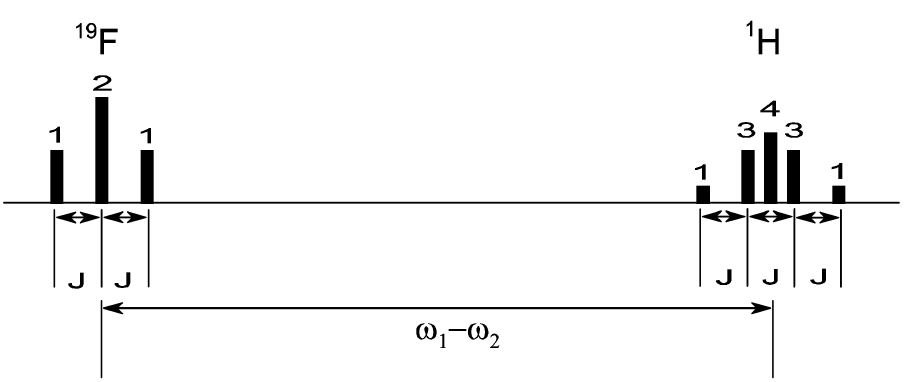
\includegraphics[width= 0.75\textwidth]{Abbildungen/JKopplungSchema.png} 
    \caption[Schematische Darstellung eines Spektrums zur veranschaulichung der erwartbaren Ergebnisse durch die Analyse der J-Kopplung. Entnommen aus \cite{Schmidt}.]{Die Abbildung zeigt schematisch ein Spektrum für Trifluoroethanol.
    Dabei ist zu erkennen, welche Erkentnisse aus dem Spektrum abgelesen werden können.
    Diese sind zum einen die Kopplungskostante $J$, welche als Abstand zwischen den Peaks eines Elements verstanden wird, zum anderen kann die Annahme der schwachen Kopplung nach Formel \eqref{eq:SchwacheKopplung} überprüft werden.
    Zudem kann aus dem Verhältnis der Peakintegrale die Verteilung der Intensitäten berechnet werden.
    Diese folgt abhängig der Anzahl der auftretenden Maxima dem \textsc{Pascal}'schen Dreieck. Entnommen aus \cite{Schmidt}.}
    \label{fig:JKSchema}
\end{figure}

Hierbei ist allerdings ein anderes Molekül -- Trifluoroethanol -- veranschaulicht.
Erkennbar ist, dass aus dem Abstand der einzelnen Peakmaxima bei Fluor und Wasserstoff die Kopplungskonstante $J$ bestimmt werden kann.
Im Falle schwacher Kopplung gilt zudem die Relation
\begin{align}
    2 \pi \cdot J \ll \vert \omega_1 - \omega_2 \vert \, , \label{eq:SchwacheKopplung}
\end{align}
zwischen Kopplungskonstante $J$ und dem Abstand der Hauptmaxima $\vert \omega_1 - \omega_2 \vert$ der beiden Elemente.
Hierbei wird angenommen, dass bei der \textsc{Zeeman}-Wechselwirkung lediglich ein Störterm erster Ordnung durch die J-Kopplung berücksichtigt werden muss.
Dieser ist proportional zu $2 \pi \cdot J$, in höheren Ordnungen trten entsprechend noch geringere Einflüsse auf, welche vernachlässigbar sind, sofern \eqref{eq:SchwacheKopplung} erfüllt ist. 
Sollten Störungen höherer Ordnung aufgrund stärkerer Kopplung vorliegen, so können diese die Peakbreite beeinflussen und vergrößern.
Zuletzt ist die Verteilung der Peakintensitäten, beziehungsweise das Verhältnis derer zueinander dargestellt.
Diese folgen, je nach Anzahl der vorliegenden Peaks pro Element, einer Verteilung nach dem \textsc{Pascal}'schen Dreieck.
Ermittelt wird diese Verteilung durch Integration über die Peaks.
Die Anzahl vorliegender Peaks ist wiederum dadurch bestimmt wie viele Spins pro Element zur Wechselwirkung beitragen.
Hat ein Element $N$ beitragende Spins, so spaltet das andere Element in $N+1$ Energieniveaus auf, welche als Peaks in der Frequenzdomäne gemessen werden können.
Entsprechend sind im vorliegenden Molekül je drei Maxima pro Element zu erwarten. \cite{Schmidt} \\

Abbildung \ref{fig:JKopplungExp} zeigt das am Versuchstag gewonnene Spektrum.
Hierbei sind farbig (blau für Fluor und grün für Wasserstoff) jeweils drei \textsc{Gauss}-Fits zu erkennen. 
Bei \SI{1750}{\hertz} ist zudem ein Peak zu erkennen, welcher, wie bereits beschrieben, auf die Taktung der deutschen Netzspannung zurückzuführen ist.

\begin{figure}[H]
    \centering
    % GNUPLOT: LaTeX picture with Postscript
\begingroup
  % Encoding inside the plot.  In the header of your document, this encoding
  % should to defined, e.g., by using
  % \usepackage[cp1252,<other encodings>]{inputenc}
  \inputencoding{cp1252}%
  \makeatletter
  \providecommand\color[2][]{%
    \GenericError{(gnuplot) \space\space\space\@spaces}{%
      Package color not loaded in conjunction with
      terminal option `colourtext'%
    }{See the gnuplot documentation for explanation.%
    }{Either use 'blacktext' in gnuplot or load the package
      color.sty in LaTeX.}%
    \renewcommand\color[2][]{}%
  }%
  \providecommand\includegraphics[2][]{%
    \GenericError{(gnuplot) \space\space\space\@spaces}{%
      Package graphicx or graphics not loaded%
    }{See the gnuplot documentation for explanation.%
    }{The gnuplot epslatex terminal needs graphicx.sty or graphics.sty.}%
    \renewcommand\includegraphics[2][]{}%
  }%
  \providecommand\rotatebox[2]{#2}%
  \@ifundefined{ifGPcolor}{%
    \newif\ifGPcolor
    \GPcolorfalse
  }{}%
  \@ifundefined{ifGPblacktext}{%
    \newif\ifGPblacktext
    \GPblacktexttrue
  }{}%
  % define a \g@addto@macro without @ in the name:
  \let\gplgaddtomacro\g@addto@macro
  % define empty templates for all commands taking text:
  \gdef\gplbacktext{}%
  \gdef\gplfronttext{}%
  \makeatother
  \ifGPblacktext
    % no textcolor at all
    \def\colorrgb#1{}%
    \def\colorgray#1{}%
  \else
    % gray or color?
    \ifGPcolor
      \def\colorrgb#1{\color[rgb]{#1}}%
      \def\colorgray#1{\color[gray]{#1}}%
      \expandafter\def\csname LTw\endcsname{\color{white}}%
      \expandafter\def\csname LTb\endcsname{\color{black}}%
      \expandafter\def\csname LTa\endcsname{\color{black}}%
      \expandafter\def\csname LT0\endcsname{\color[rgb]{1,0,0}}%
      \expandafter\def\csname LT1\endcsname{\color[rgb]{0,1,0}}%
      \expandafter\def\csname LT2\endcsname{\color[rgb]{0,0,1}}%
      \expandafter\def\csname LT3\endcsname{\color[rgb]{1,0,1}}%
      \expandafter\def\csname LT4\endcsname{\color[rgb]{0,1,1}}%
      \expandafter\def\csname LT5\endcsname{\color[rgb]{1,1,0}}%
      \expandafter\def\csname LT6\endcsname{\color[rgb]{0,0,0}}%
      \expandafter\def\csname LT7\endcsname{\color[rgb]{1,0.3,0}}%
      \expandafter\def\csname LT8\endcsname{\color[rgb]{0.5,0.5,0.5}}%
    \else
      % gray
      \def\colorrgb#1{\color{black}}%
      \def\colorgray#1{\color[gray]{#1}}%
      \expandafter\def\csname LTw\endcsname{\color{white}}%
      \expandafter\def\csname LTb\endcsname{\color{black}}%
      \expandafter\def\csname LTa\endcsname{\color{black}}%
      \expandafter\def\csname LT0\endcsname{\color{black}}%
      \expandafter\def\csname LT1\endcsname{\color{black}}%
      \expandafter\def\csname LT2\endcsname{\color{black}}%
      \expandafter\def\csname LT3\endcsname{\color{black}}%
      \expandafter\def\csname LT4\endcsname{\color{black}}%
      \expandafter\def\csname LT5\endcsname{\color{black}}%
      \expandafter\def\csname LT6\endcsname{\color{black}}%
      \expandafter\def\csname LT7\endcsname{\color{black}}%
      \expandafter\def\csname LT8\endcsname{\color{black}}%
    \fi
  \fi
    \setlength{\unitlength}{0.0500bp}%
    \ifx\gptboxheight\undefined%
      \newlength{\gptboxheight}%
      \newlength{\gptboxwidth}%
      \newsavebox{\gptboxtext}%
    \fi%
    \setlength{\fboxrule}{0.5pt}%
    \setlength{\fboxsep}{1pt}%
\begin{picture}(7200.00,5040.00)%
    \gplgaddtomacro\gplbacktext{%
      \csname LTb\endcsname%%
      \put(814,704){\makebox(0,0)[r]{\strut{}$0$}}%
      \put(814,1218){\makebox(0,0)[r]{\strut{}$0.5$}}%
      \put(814,1733){\makebox(0,0)[r]{\strut{}$1$}}%
      \put(814,2247){\makebox(0,0)[r]{\strut{}$1.5$}}%
      \put(814,2762){\makebox(0,0)[r]{\strut{}$2$}}%
      \put(814,3276){\makebox(0,0)[r]{\strut{}$2.5$}}%
      \put(814,3790){\makebox(0,0)[r]{\strut{}$3$}}%
      \put(814,4305){\makebox(0,0)[r]{\strut{}$3.5$}}%
      \put(814,4819){\makebox(0,0)[r]{\strut{}$4$}}%
      \put(946,484){\makebox(0,0){\strut{}$1700$}}%
      \put(2410,484){\makebox(0,0){\strut{}$1750$}}%
      \put(3875,484){\makebox(0,0){\strut{}$1800$}}%
      \put(5339,484){\makebox(0,0){\strut{}$1850$}}%
      \put(6803,484){\makebox(0,0){\strut{}$1900$}}%
    }%
    \gplgaddtomacro\gplfronttext{%
      \csname LTb\endcsname%%
      \put(308,2761){\rotatebox{-270}{\makebox(0,0){\strut{}Amplitude in $\si{\milli \second}$}}}%
      \put(3874,154){\makebox(0,0){\strut{}Frequenz in $\si{\hertz}$}}%
      \csname LTb\endcsname%%
      \put(5816,4646){\makebox(0,0)[r]{\strut{}Messung zur J-Kopplung}}%
      \csname LTb\endcsname%%
      \put(5816,4426){\makebox(0,0)[r]{\strut{}\textsc{Lorentz}-Fit}}%
    }%
    \gplbacktext
    \put(0,0){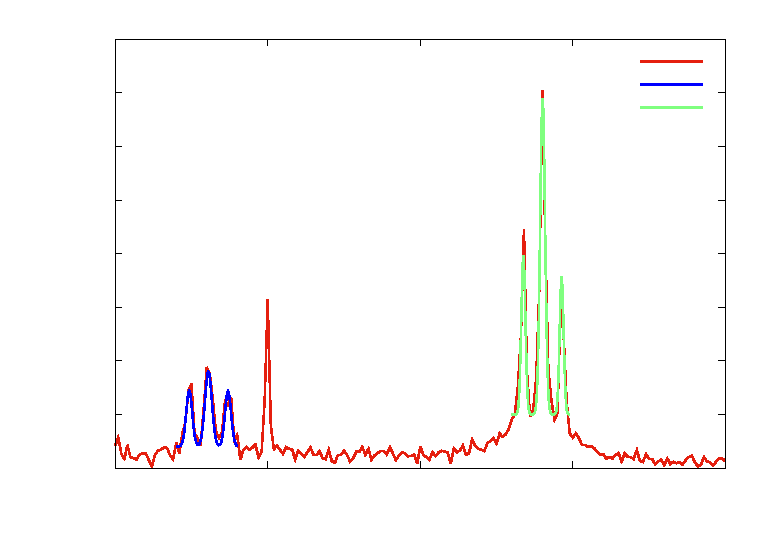
\includegraphics{plots/JKopplung}}%
    \gplfronttext
  \end{picture}%
\endgroup

    \caption[Spektrum zur Analyse der J-Kopplung zwischen Fluor und Wasserstoff.]{Die Abbildung zeigt das am Versuchstag aufgenommene Spektrum, welches Rückschlüsse auf die J-Kopplung zwischen Fluor und Wasserstoff zulässt. 
    Dabei wurden je drei Peaks von Fluor und Wasserstoff mittels einer \textsc{Gauss}-Funktion gefittet um die Lage des Maximums, die Standardabweichung und die Fläche unterhalb des Peaks als Fitparameter zu gewinnen.
    Diese gewonnen Werte wurden dann verwendet um die Kopplungskonstante $J = \SI{6.3 \pm 1.3}{\hertz}$ zu berechnen, die Frage zu beantworten, ob schwache J-Kopplung vorliegt und die Verhältnisse der Peaks zu analysieren.}
    \label{fig:JKopplungExp}
\end{figure}

Durch die \textsc{Gauss}-Fits konnten sowohl die Lage der Maxima, die Peakbreiten sowie die Integrale der Peaks berechnet werden.
Dabei wurde zudem die jeweilige Standardabweichung $\sigma$ als Fitparameter gewonnen, welche in Folge als Unsicherheit der Peakposition herangezogen wurde.
Die Integrale der Peaks konnten dabei dadurch berechnet werden, dass das Integral über die \textsc{Gauss}'sche-Dichtefunktion
\begin{align}
    \frac{1}{\sqrt{2 \pi \sigma^2}} \exp{\left(-\frac{\left(x-\mu\right)^2}{2 \sigma^2}\right)}
\end{align}
auf $1$ normiert ist.
Diese wurde als Fitfunktion herangezogen.
Dabei beschreibt $\sigma$ die Standardabweichung, $\mu$ die Position des Maximums. Wird ein zusätzlicher Faktor $b$ berücksichtigt, so gibt dieser den Wert des Integrals in guter Näherung an.

Somit ergaben sich für die Kopplungskonstanten folgende gewichtete Mittelwerte mit der jeweils zugehörigen kombinierten Unsicherheit, welche aus der jeweiligen Standardabweichung fortgeführt wurde:
\begin{align*}
    J_{\text{F}} = \SI{6.4 \pm 1.1}{\hertz} \\
    J_{\text{H}} = \SI{6.27 \pm 0.74}{\hertz} \\
    J_{\text{MW}} = \SI{6.3 \pm 1.3}{\hertz}.
\end{align*}
Da $J_{\text{F}}$ und $J_{\text{H}}$ ohnehin übereinstimmen sollten, bestätigen sich die berechneten Werte gegenseitig.
Zudem wurde eine Kopplungskonstante von $\SI{6}{\hertz}$ auf Grundlage der am Versuchstag vorliegenden Gegebenheiten erwartet.
Entsprechend bestätigen die Ergebnisse hier die Vorhersagen.
Die berechneten Unsicherheiten liegen zudem in einer sinnvollen Größenordnung und unterstreichen die Genauigkeit der Ergebnisse.

Bezüglich der Annahme der schwachen Kopplung konnte der Abstand der Hauptmaxima $\vert \omega_1 - \omega_2 \vert$ bestimmt werden und die Hypothese mittels Relation \eqref{eq:SchwacheKopplung} überprüft werden.
Hierbei ergab sich folgender Zusammenhang:
\begin{align*}
    2 \pi \cdot \SI{6.3}{\hertz} &\ll \vert \SI{1730}{\per \second} - \SI{1840}{\per \second} \vert \\
    <\approx > \quad \SI{6}{\hertz} &\ll \SI{18}{\hertz}
\end{align*}
Dabei genügt es ein Abschätzung vorzunehmen, weswegen keine exakten Werte berechnet wurden und auch auf die Angabe der Unsicherheiten verzichtet wurde.
Hierbei ist zu konstatieren, dass die Kopplungskonstante zwar kleiner als der Abstand der Hauptmaxima ist, jedoch nicht signifikant.
Die Annahme der schwachen Kopplung kann folglich nicht bestätigt werden.
Daher ist -- wie oben beschrieben -- mit einem Aufweiten der Peaks im Spektrum zu rechnen, was sich auch in den Werten der Peakintegrale widerspiegeln sollte.
Dieses Aufweiten ist erwartbar, da bei stärkere Kopplung eine feinere Aufspaltung der in mehr Maxima erwartet wird.
Diese können aber nicht zwangsläufig separat aufgelöst werden, weswegen sich der Effekt als Aufweiten der Peaks erkennen lässt.
\begin{table}[H]
    \centering
    \caption{Übersicht über die berechneten relativen Peakintegrale der J-Kopplung.}
    \begin{tabular}{|l||r|r|r|} \hline
        Element & Peakposition in \si{\hertz} & rel. Peakintegral & Standardabweichung $\sigma$ \\ \hline \hline
        Fluor & \SI{1724.3 \pm 1.0}{} & \SI{1 \pm 0.63}{} & \SI{1.0}{}\\ \hline
        Fluor & \SI{1730.6 \pm 1.1}{}& \SI{1.54 \pm 0.54}{} & \SI{1.1}{}\\ \hline
        Fluor & \SI{1737.0 \pm 1.0}{} &\SI{1 \pm 0.41}{}& \SI{1.0}{}\\ \hline \hline
        Wasserstoff & \SI{1833.79 \pm 0.67}{} & \SI{1 \pm 0.55}{}& \SI{0.67}{}\\ \hline
        Wasserstoff & \SI{1840.11 \pm 0.81}{} & \SI{2.4 \pm 0.77}{}& \SI{0.81}{}\\ \hline
        Wasserstoff & \SI{1846.34 \pm 0.65}{}  & \SI{0.84 \pm 0.39}{}& \SI{0.65}{}\\ \hline
    \end{tabular} 
    \label{tab:Peaksintens} 
\end{table}
Tabelle \ref{tab:Peaksintens} zeigt eine Übersicht über die relativen Peakintegrale.
Dabei wurden die relativen Integrale jeweils auf den Wert des Maximums welches bei der geringsten Frequenz auftrat normiert.
Die angegebenen Unsicherheiten sind dabei durch die Standardabweichung gegeben, welche als Fitparameter \textit{GnuPlot} entnommen und nach der Formel zur kombinierten Unsicherheit fortgeführt wurde.
Nun zeigt sich grundsätzlich -- unter Berücksichtigung der recht groß ausfallenden Unsicherheiten -- eine Verteilung der Peaks nach dem \textsc{Pascal}'schen Dreieck (1:2:1).
Allerdings sind die Abweichungen der tatsächlichen Werte der relativen Peakintegrale von der Verhältnismäßigkeit (1:2:1) doch recht groß.
Die absoluten Werte lassen somit ebenfalls darauf schließen, dass die Annahme der schwachen Kopplung nicht erfüllt sein könnte.
Die Abweichungen von der Verhältnismäßigkeit (1:2:1) lassen vermuten, dass die Peaks tatsächlich aufgeweitet auftreten.
Bei Fluor würde dies die beiden Nebenmaxima betreffen, bei Wasserstoff könnte vor allem das Hauptmaximum beroffen sein.
Unterstrichen wird dies durch die Betrachtung der Standardabweichung der Peaks in Tabelle \ref{tab:Peaksintens}. 
Insbesondere bei Wasserstoff liegt offenbar ein Unterschied bei der Standardabweichung zwischen dem Haupt- und den Nebenmaxima vor.
Dieser Unterschied in der Peakweite, welcher durch $\sigma$ charakterisiert wird belegt das Aufweiten der Peaks.
Zudem wurde während der Versuchsdurchführung versucht ein möglichst rauschfreies Spektrum mit recht eindeutigen Maxima zu erhalten.
Um dies zu gewährleisten wurde die Anzahl der aufgenommenen Datenpunkte reduziert.
Dies führt dazu, dass pro Fit nur wenige Datenpunkte erfasst werden konnten.
Dadurch liegt der Schluss nahe, dass zum einen die angegebenen Unsicherheiten womöglich zu klein ausfallen und zum anderen hätten mehr Datenpunkte zu verlässlicheren Ergebnissen geführt.
Die Abweichungen in den Peakintegralen könnten folglich auch von diesem Umstand beeinflusst sein.
Insgesamt kann also festgehalten werden, dass vor allem bei der Betrachtung der Kopplungskonstante gute Übereinstimmungen mit der Theorie beziehungsweise den Erwartungen erzielt wurden.
Zudem ließen die Betrachtung der schwachen Wechselwirkung und der Peakintegrale interessante Rückschlüsse zu und förderten eine kritische Auseinandersetzung mit selbigen, auch wenn die quantitativen Betrachtung durchaus den Schluss zulassen, dass Optimierungen am Versuchsaufbau und während der Durchführung denkbar sind.



